\documentclass[11pt, twoside, reqno]{article}
\usepackage{amssymb, amsthm, amsmath, amsfonts}
\usepackage{graphicx}
\usepackage{color}
\usepackage{hyperref}
\usepackage{verbatim}
\usepackage[toc,page]{appendix}
\usepackage{listings}
\usepackage[shortlabels]{enumitem}
\setlist[enumerate, 1]{1\textsuperscript{o}}

\definecolor{codegreen}{rgb}{0,0.6,0}
\definecolor{codegray}{rgb}{0.5,0.5,0.5}
\definecolor{codepurple}{rgb}{0.58,0,0.82}
\definecolor{backcolour}{rgb}{0.95,0.95,0.92}

\lstdefinestyle{mystyle}{
    backgroundcolor=\color{backcolour},
    commentstyle=\color{codegreen},
    keywordstyle=\color{magenta},
    numberstyle=\tiny\color{codegray},
    stringstyle=\color{codepurple},
    basicstyle=\footnotesize,
    breakatwhitespace=false,
    breaklines=true,
    captionpos=b,
    keepspaces=true,
    numbers=left,
    numbersep=5pt,
    showspaces=false,
    showstringspaces=false,
    showtabs=false,
    tabsize=2
}

\lstset{style=mystyle}

\begin{document}

\label{label}
\section{Introduction}
\hspace{0.1in} Just under three million tweets were collected for this experiment. These tweets were streamed from Twitter through a collection pipeline and stored in a Database in the weeks leading up to the Midterm Election. The pipeline was organized as such:

\begin{figure}[h]
	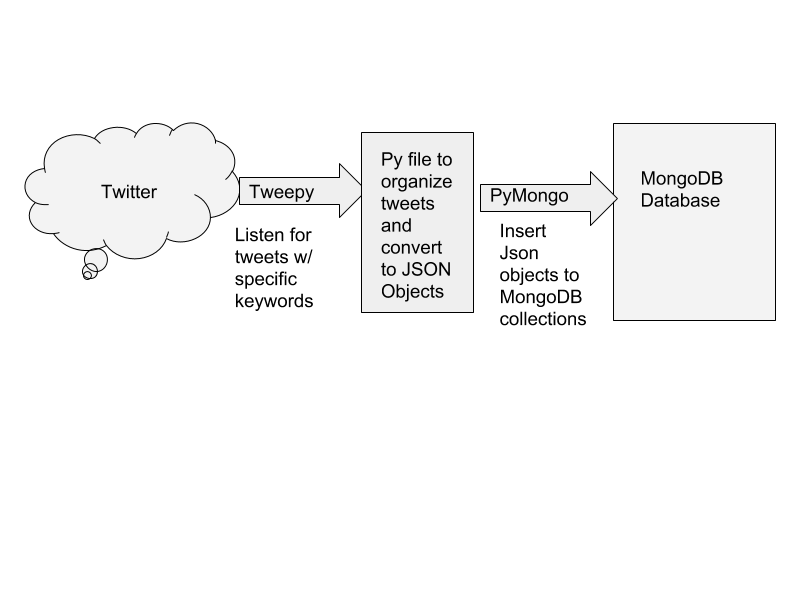
\includegraphics[scale=0.5]{data_collection}
\end{figure}

Building the pipeline consisted of three distinct tasks. 
\begin{enumerate}
	\item Building a tweet streamer to "listen" to tweets based on keywords
	\item Preprocessing the tweets
	\item Storing processed tweets in a database. 
\end{enumerate}
All the code written to built the pipeline can be found in Appendix A.


\section{Streaming Tweets}
\hspace{0.1in} There are two ways to gather tweets using the Python Twitter API (Applications Package Interface). One is to query a profile or a search term. This method is not preferred for several reasons. First, Twitter has put a hard cap on the number of tweets each query can return at one time. This means that querying will be in-exact and time consuming loop. Next, Twitter's search function will naturally promote tweets that have more engagement. This means that tweets with more likes and retweets, comments, and followers will get preference, which results in a biased data set. 

The other way to gather tweets is to stream tweets. A Tweepy stream monitors live twitter content and returns all tweets that contain a given set of keywords. Streaming has the disadvantage of gathering only live tweets - it does not search tweets from before it started running. But, streaming has the advantage of gathering any tweets that meet the keyword requirement, irrelevant of engagement. Consequently, it was decided that the tweets gathered would be through streaming. 

The streamer is abstracted in the Twitter API. To use it, the user must define the actual methods the streamer needs to find and save tweets. The methods defined here are on\_connect, on\_error, and on\_data. The first two are trivial. On\_connect is used to connect, and confirms once the stream is live. If the stream crashes - which can happen for several reasons - on\_error informs the user why the stream stopped (memory, exceeding latency, etc.). The last method on\_data is where the tweets are received and processed. Each tweet is received as a dictionary data structure where keys are attributes of the tweet (i.e. date and time, text, user, etc.). From there any processing is up to the user; the tweet's text can be printed, the tweets can be prepared for entry to a data base, etc. It's here that the tweets will be modified to fit MongoDB's insertion requirements. 

\section{Databases}
\hspace{0.1in} The tweets that the Tweepy streams need to be stored. An Excel file is a convenient but imperfect solution. A database will take full advantage of the object stored as well as the large data set in question. 
\subsection{Overview}
The term database refers to any structure that electronically stores data. In extension, the Database Management System is the program that allows users to interact with the database. In this paper, when the term database is used, it refers to both the structure and the system. 

There are several types of databases. These types are classified by the way the data is organized inside the structure. The relational database model uses tables with rows and columns to store information. Relational databases use SQL to organize, extract, and insert data. Non-relational databases, referred to colloquially to as "NoSQL" use an object-oriented approach with different query languages. 

Databases offer several advantages that other storage options like Excel or CSVs will not. The ability to quickly search and sort through millions of tweets as well as the flexibility to manipulate said data is something that isn't available to Excel. Additionally these databases have organized and maintained APIs for Python. 

\subsection{MongoDB}
\hspace{0.1in} MongoDB is a popular non-relational database management system thats's offered for free. It has an efficient query language as well as a well-defined API Pymongo. In a MongoDB database, each tweet is an object. These objects are stored in collections and the collections are stored in a database:

\begin{figure}[h]
	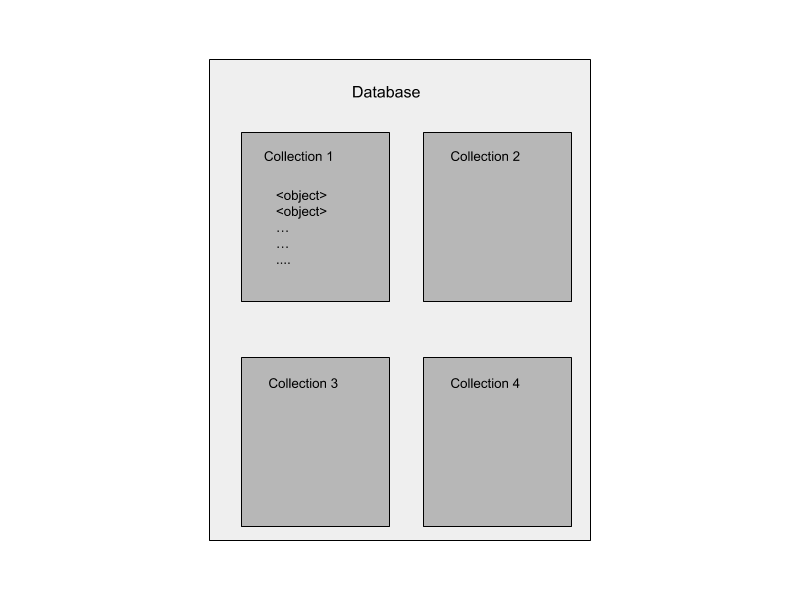
\includegraphics[scale=0.5]{database}
\end{figure}

These JSON objects have fields, populated with values. MongoDB allows a user to query collections using field values. These queries can be exact matches or other operators. For example, you can query tweets by date, or location (by exact match). You can also query sub-matches. That means conditions within a field and not an exact match, like searching for all tweets that contain Donald Trump.

MongoDB has a mongoshell through which a user can interact with the databases. For longer and larger actions, we use the Python API Pymongo to write python scripts. Pymongo allows us to insert, edit, and query databases and manipulate the output. 

For more specifics on Pymongo and setting up MongoDB, refer to the Appendix or the Pymongo documentation.

\section{Data Collection}
\hspace{0.1in} 
Implementing the pipeline referred to earlier means that tweets are streamed and inserted into a MongoDB Database. The first step of streaming requires search terms. These search terms were taken from house and senate races, as well as general terms that refer to the 2018 midterms. Search terms for Senate and House Races were tweets about the candidates as well as a hashtag referring to the race. 

To direct the tweets streamed into a database, the on\_data method is defined. This method is designed for the streamer to deal with the tweets it selects.

\begin{verbatim}
def on_data(self, data):
	try:
            client = MongoClient(MONGO_HOST)

            # Use twitterdb database. If it doesn't exist, it will be created.
            db = client.miscdb

            # Decode the JSON from Twitter
            datajson = json.loads(data)

            #grab the 'created_at' data from the Tweet to use for display
            created_at = datajson['created_at']

            #print out a message to the screen that we have collected a tweet
            print("Tweet collected at " + str(created_at) + " " + datajson['text'])

            #insert the data into the mongoDB into a collection called twitter_search
            #if twitter_search doesn't exist, it will be created.
            db.misc.insert(datajson)
        except Exception as e:
           print(e)
\end{verbatim}

The tweet is converted into a JSON object - MongoDB's preferred type - and inserted into a database and collection of the users choice. This is a barebones definition. Sorting, editing, and adding information to tweets would all be defined here. For the entire script that streamed tweets for the senate or the house, refer to Appendix A.

The data collection process ran through three separate scripts each with a different set of search terms. Those three scripts fed into three different collections in a massive database. Together they assemble a diverse dataset that contains just under three million tweets. Chapter <insert number here> will explore the dataset we've assembled. 

\end{document}

